% Provenance (never printed): cycle 4 SVT/physique, "La planete Terre,
% l'environnement": the atmosphere, its structure and its layers, pressure
% and altitude, the ozone layer; see sources/book1/PROVENANCE.md. Book 1,
% grade 8, chapter 1.
% Vocabulary guard: owns the layers of the atmosphere (troposphere,
% tropopause, stratosphere, mesosphere, thermosphere), the environmental
% lapse rate and the ozone layer. Air pressure and the barometer are the
% physics books' (recalled), the composition of air and ozone the molecule
% the chemistry books'; "convection cell" is g8.2's and is not used here;
% adiabatic cooling is Book 2's.
\chapter{大气}\label{ch:g8:the-atmosphere}

在一个\omterm{def:g4:clouds-rain-snow:weather-station}{气象站}，约定时刻之前，一位气象学家走到草地上，
手里拿着一只充满氢气或氦气的气球，直径约
\qty{1.5}{m}。气球下方的长绳上挂着一个小橙色降落伞和一个重 60 至 80 克的仪器盒：
\emph{探空仪}。
她松手放飞。气球每分钟约上升 \qty{300}{m}，探空仪每
秒都向地面发回气压、温度、
湿度和自身位置。随着上升，气球不断膨胀，直到
直径达到 6 至 \qty{8}{m} 时破裂，通常在 \qty{30}{km} 以上的高空，
即放飞后约两小时。每天的同一时刻，
全球 800 多个站点同时上演同样的情景。
% ledger: nws:radiosonde

\begin{omfigure}
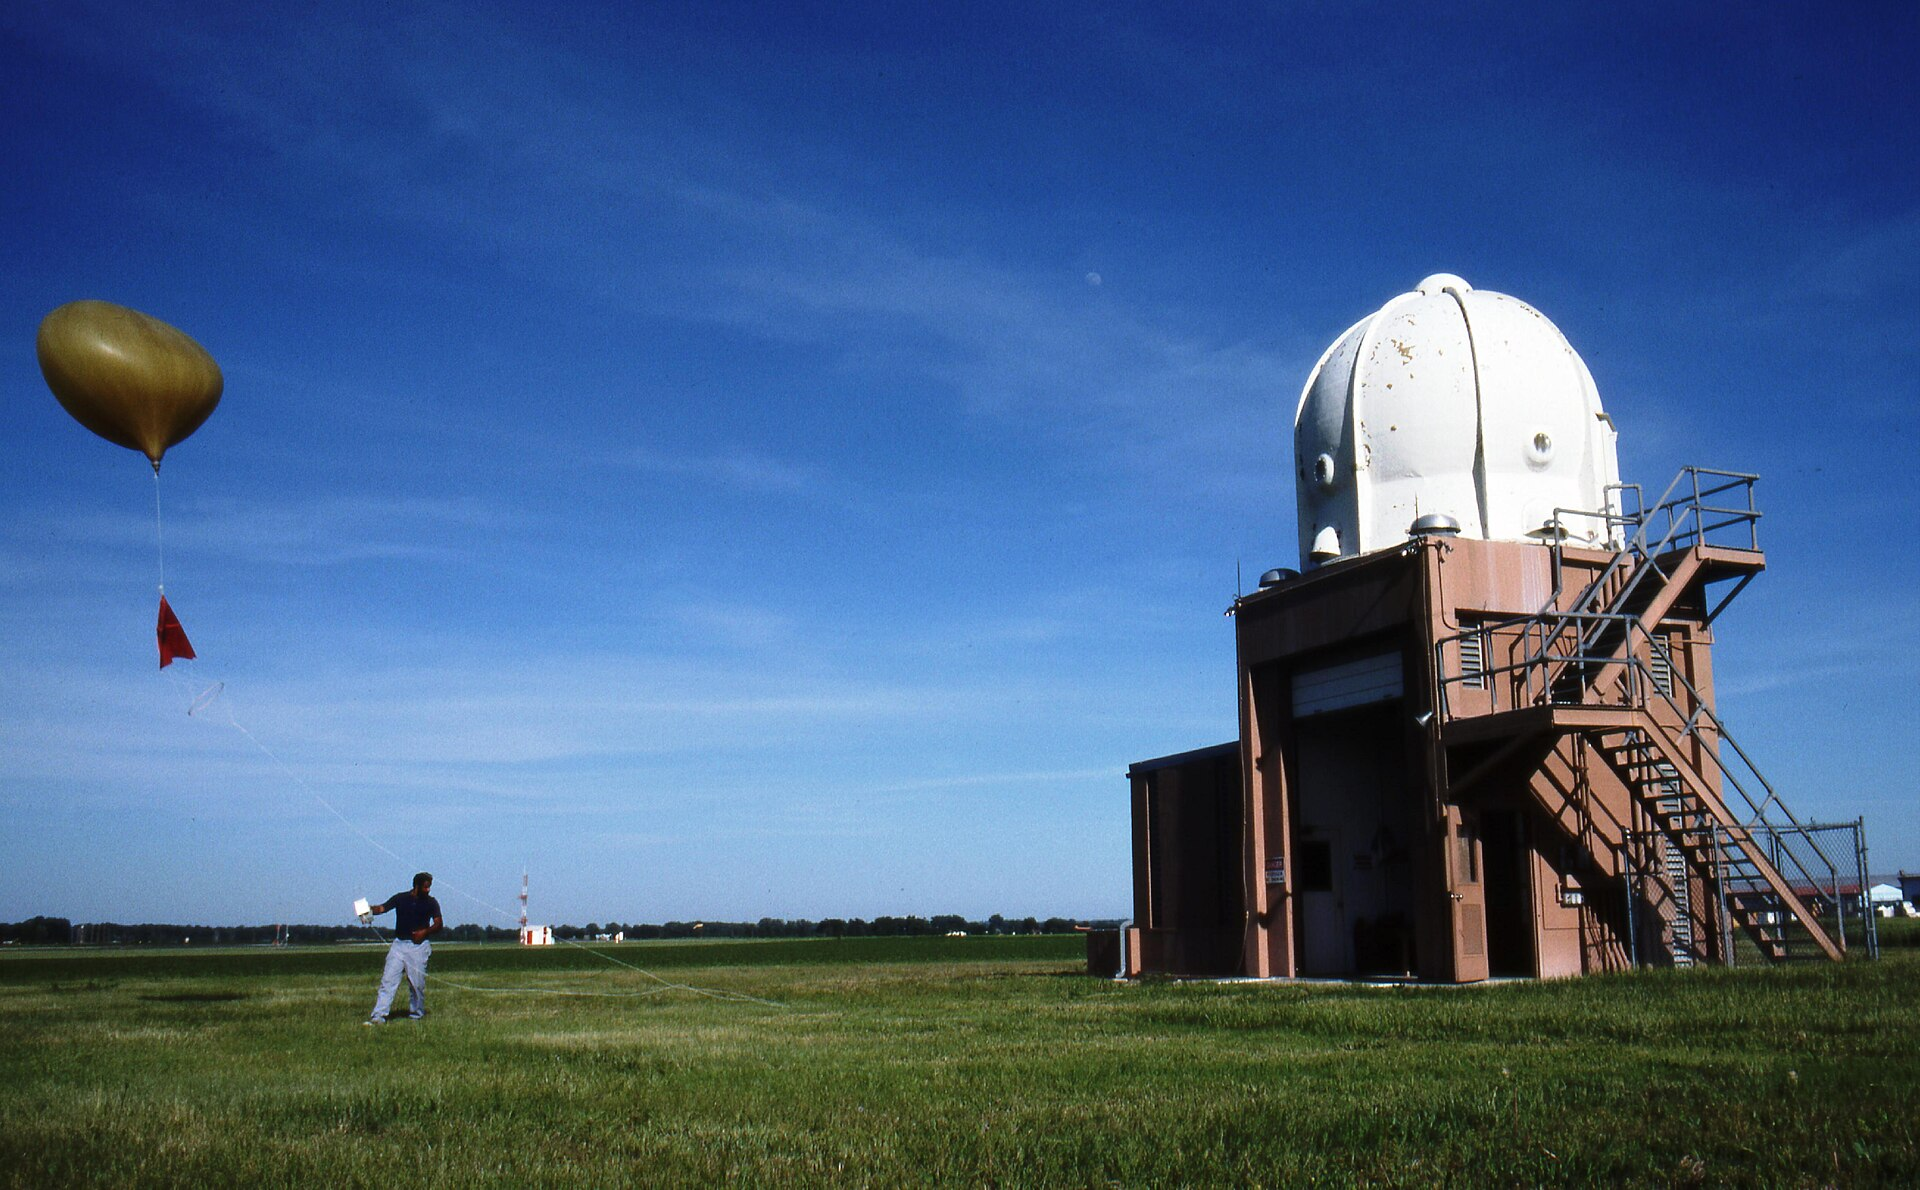
\includegraphics[width=0.78\linewidth]{images/book1/g8-radiosonde-launch.jpg}

{\small 在美国堪萨斯州托皮卡放飞气象气球：
红色降落伞和探空仪悬挂在气球下方。照片由
Stephen Corfidi 拍摄，NOAA/National Weather Service（公有领域，
经由维基共享资源）。}
% ledger: commons:radiosonde-launch
\label{fig:g8:the-atmosphere:launch}
\end{omfigure}

为什么气球随着上升会膨胀？探空仪在上升途中测量什么，
以及为什么温度不会简单地一直下降？大气
的上界在哪里？

\begin{recall}
\emph{大气}是包围地球的空气层。空气
会压在接触到的一切物体上：这就是\emph{气压}，可用气压计测量
（物理学中的内容）。气象部门以百帕
（hPa）为单位给出；\omterm{def:g4:world-physical-map:altitude}{海平面}气压约为 \qty{1013}{hPa}。干燥空气中
约 78~\% 为氮气，21~\% 为氧气，
另含少量氩气、二氧化碳及其他气体（化学中的内容）。云
由微小的水滴或冰晶构成（见\cref{ch:g4:clouds-rain-snow}）。
\end{recall}
% ledger: air:N2, air:O2, ussa76:sea-level

\section{薄薄的大气层}

从国际空间站望去，大气是沿地球边缘的一道
发光细线。大部分空气和几乎全部的云
都集中在其最底层的几千米之内。
% ledger: commons:iss-sunset

\begin{omfigure}
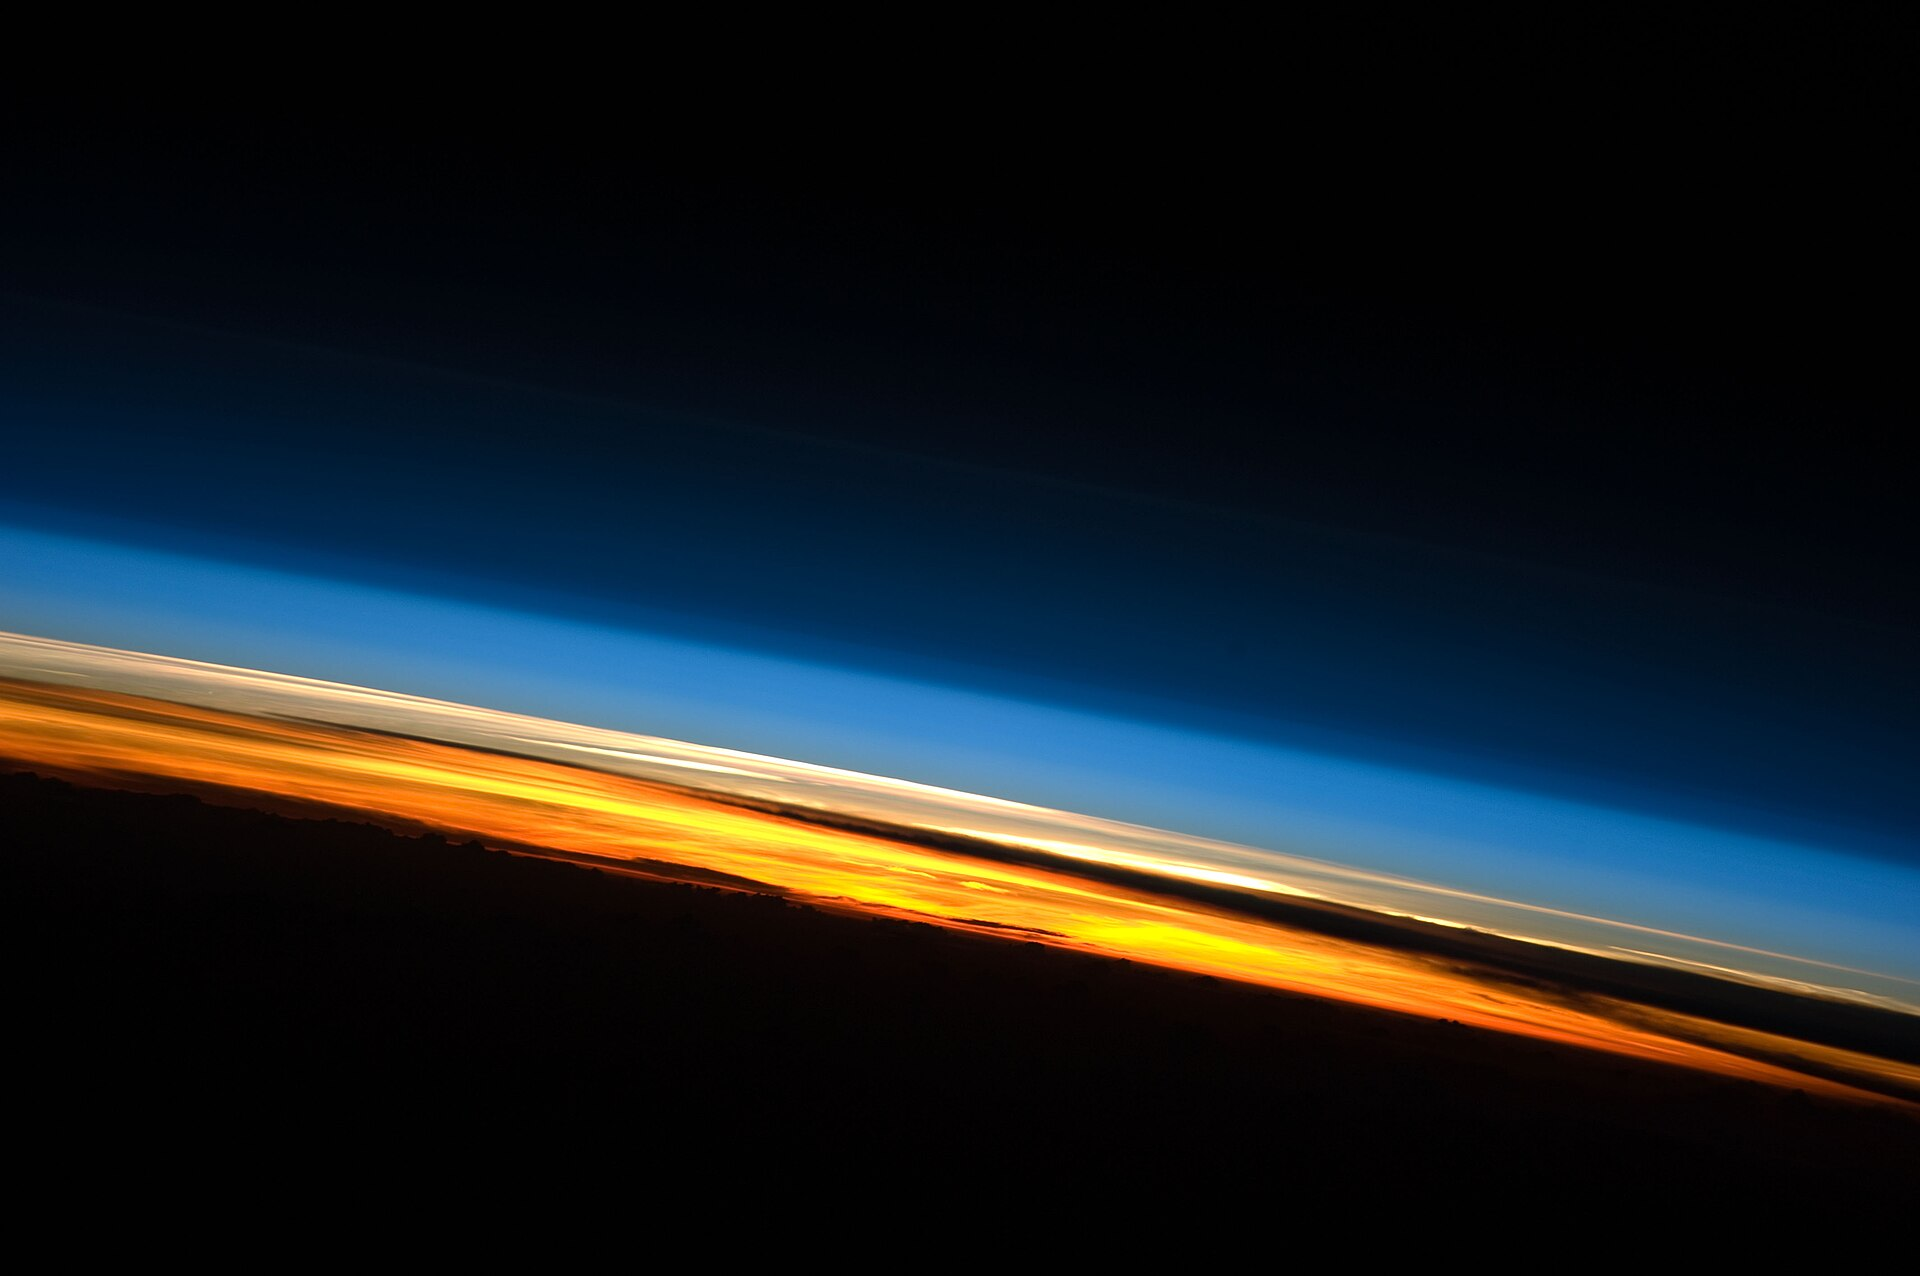
\includegraphics[width=0.78\linewidth]{images/book1/g8-iss-limb.jpg}

{\small 2010 年 6 月 14 日，日落时分，国际空间站
在印度洋上空拍摄的地球边缘。图中橙色和黄色的带状部分是大气的最底层，
其中有深色的云；其上是颜色渐淡、继而呈蓝色的各层，
逐渐融入太空的漆黑之中。NASA 照片，
ISS Expedition~23（公有领域，经由
维基共享资源）。}
% ledger: commons:iss-sunset
\label{fig:g8:the-atmosphere:limb}
\end{omfigure}

大气并没有明确的上界，空气
随高度增加而越来越稀薄。按惯例，太空始于约 \qty{100}{km} 处。
与地球半径 \qty{6371}{km} 相比，这一比值很小：$100 \div
6371 \approx 0.016$，不到半径的 2~\%。在
一个直径为 \qty{30}{cm} 的\omterm{def:g3:continents-and-oceans:globe}{地球仪}上，整个大气层就像一层约
\qty{2}{mm} 厚的薄膜。
% ledger: ucar:layers, earth:Rmean

\begin{omfigure}
\begin{tikzpicture}[font=\footnotesize]
  % 1 cm = 100 km: the Earth's surface is a circle of radius 63.71 cm
  \def\R{63.71}
  \useasboundingbox (-6.9,-1.6) rectangle (6.9,1.0);
  \fill[blue!8] (0,-\R) ++(85:\R+1) arc (85:95:\R+1) -- ($(0,-\R)+(95:\R)$) arc (95:85:\R) -- cycle;
  \fill[omLithAlluv!70] (0,-\R) ++(85:\R) arc (85:95:\R) -- ++(0,-0.6) -- ($(0,-\R)+(85:\R)+(0,-0.6)$) -- cycle;
  \draw[black, line width=0.6pt] (0,-\R) ++(85:\R) arc (85:95:\R);
  \foreach \h/\c in {0.1102/omThm, 0.4938/omMeth, 0.86/omDef} \draw[\c, line width=0.5pt] (0,-\R) ++(85:\R+\h) arc (85:95:\R+\h);
  \draw[black!60, dashed] (0,-\R) ++(85:\R+1) arc (85:95:\R+1);
  \node[anchor=west, omThm] at (5.65,-0.14) {\qty{11}{km}};
  \node[anchor=west, omMeth] at (5.65,0.25) {\qty{49}{km}};
  \node[anchor=west, omDef] at (5.65,0.62) {\qty{86}{km}};
  \node[anchor=east, black!70] at (-5.65,0.75) {\qty{100}{km}};
  \node[anchor=north] at (0,-0.15) {地球表面};
  \draw[|-|] (-5,-1.05) -- node[below] {\qty{1000}{km}} (5,-1.05);
\end{tikzpicture}

{\small 按比例绘制的地球及其大气剖面图（
\qty{1}{cm} 代表 \qty{100}{km}），画至 \qty{100}{km}，即太空边缘（虚线）。
彩色线条标出本章后面将介绍的各层
边界。最底层是\omterm{def:g1:watching-the-weather:weather}{天气}现象都发生的地方，
厚度仅约一毫米。}
% ledger: earth:Rmean, ucar:layers (limits: figdata/grade-8/standard_atmosphere.py main table)
\label{fig:g8:the-atmosphere:to-scale}
\end{omfigure}

\section{气压随海拔降低}

大气底部的空气承受着其上方全部空气的重量。
\omterm{def:g4:world-physical-map:altitude}{海拔}越高，头顶的空气越少，气压就越低。
气象学家和工程师使用的标准大气模型中，
\omterm{def:g4:world-physical-map:altitude}{海平面}气压为 \qty{1013}{hPa}，
约 \qty{5.5}{km} 高处的气压为其一半，
约 \qty{10.3}{km} 高处为其四分之一。
% ledger: ussa76:sea-level, ussa76:layers (figdata/grade-8/standard_atmosphere.py main table: half_km 5.48, quarter_km 10.29)

由于气压度量的是其上方空气的重量，半压高度
也就是低于它的空气恰好占一半的高度：大气的一半被压缩在最底下的
\qty{5.5}{km} 之内。\qty{11}{km} 以下约有 78~\% 的空气，
\qty{30}{km} 以下约有 99~\% 的空气。
% ledger: (computed: figdata/grade-8/standard_atmosphere.py, share_below_11km 77.7, share_below_30km 98.82)

\begin{omfigure}
\begin{minipage}[t]{0.49\linewidth}\centering
\begin{tikzpicture}
\begin{axis}[width=6.6cm, height=7.6cm, xmin=0, xmax=1100, ymin=0, ymax=30,
  xlabel={气压（hPa）}, ylabel={海拔（km）},
  tick label style={font=\scriptsize}, label style={font=\small},
  xtick={0,250,500,750,1000}, ytick={0,5,10,15,20,25,30}]
  \addplot[dashed, black!60] table {figdata/out/grade-8-standard_atmosphere-guides.dat};
  \addplot[omDef, line width=1.1pt] table[x=p_hPa, y=z_km] {figdata/out/grade-8-standard_atmosphere-pressure.dat};
  \addplot[only marks, mark=*, mark size=1.8pt, omThm, point meta=explicit symbolic]
    table[x=p_hPa, y=z_km, meta=label] {figdata/out/grade-8-standard_atmosphere-levels.dat};
  \node[omThm, anchor=south west, font=\scriptsize, text=black] at (axis cs:506.6,5.48) {一半};
  \node[omThm, anchor=south west, font=\scriptsize, text=black] at (axis cs:253.3,10.29) {四分之一};
\end{axis}
\end{tikzpicture}

{\small 气压随\omterm{def:g4:world-physical-map:altitude}{海拔}变化。气压为\omterm{def:g4:world-physical-map:altitude}{海平面}值一半时的\omterm{def:g4:world-physical-map:altitude}{海拔}约为
\qty{5.5}{km}，为四分之一时约为 \qty{10.3}{km}。}
\end{minipage}\hfill
\begin{minipage}[t]{0.49\linewidth}\centering
\begin{tikzpicture}[font=\footnotesize]
  % at launch: 1.5 m; at burst: about 7 m (drawn 1 cm for 1.5 m)
  \draw[black!60] (0,0.9) -- (0,2.6);
  \shade[ball color=yellow!60!brown] (0,3.1) circle (0.5);
  \fill[red!75] (-0.25,1.75) .. controls (-0.2,2.05) and (0.2,2.05) .. (0.25,1.75) -- cycle;
  \fill[white, draw=black] (-0.15,0.55) rectangle (0.15,0.9);
  \node[anchor=north] at (0,0.45) {发射时};
  \node[anchor=north] at (0,0.05) {直径 \qty{1.5}{m}};
  \begin{scope}[xshift=3.1cm]
    \draw[black!60] (0,0.9) -- (0,2.6);
    \shade[ball color=yellow!40!white] (0,4.9) circle (2.3);
    \fill[red!75] (-0.25,1.75) .. controls (-0.2,2.05) and (0.2,2.05) .. (0.25,1.75) -- cycle;
    \fill[white, draw=black] (-0.15,0.55) rectangle (0.15,0.9);
    \node[anchor=north] at (0,0.45) {即将破裂前};
    \node[anchor=north] at (0,0.05) {直径 6 至 \qty{8}{m}};
  \end{scope}
  \node[anchor=west, font=\scriptsize] at (0.3,1.9) {降落伞};
  \node[anchor=west, font=\scriptsize] at (0.3,0.72) {探空仪};
\end{tikzpicture}

{\small 气球上升时体积膨胀，因为周围空气的
压强越来越小（气球与降落伞按相互比例绘制，
绳子已缩短）。}
% ledger: nws:radiosonde
\end{minipage}
% ledger: ussa76:sea-level, ussa76:layers (figdata/grade-8/standard_atmosphere.py parts pressure, levels, guides)
\label{fig:g8:the-atmosphere:pressure}
\end{omfigure}

再往高处，气压继续下降，每升高几千米约减半，
因此很快变得极小。用 10 的幂次表示最为方便。
在 \qty{30}{km} 高处，气压约为 \qty{12}{hPa}，
约为\omterm{def:g4:world-physical-map:altitude}{海平面}气压的 $10^{-2}$（即百分之一）；在 \qty{50}{km} 高处，约为
\qty{0.8}{hPa}，约为 $10^{-3}$；在 \qty{80}{km} 高处，约为
\qty{0.01}{hPa}，约为\omterm{def:g4:world-physical-map:altitude}{海平面}气压的 $10^{-5}$。
% ledger: ussa76:layers (figdata/grade-8/standard_atmosphere.py main table: p_30km 11.97, p_50km 0.798, p_80km 0.0105 hPa)

\begin{omfigure}

\includegraphics[width=0.5\linewidth]{images/book1/ai/g8-climbers.jpg}

{\small 登山者在极高的山上背着氧气瓶。在
\qty{9}{km} 高处，气压不足\omterm{def:g4:world-physical-map:altitude}{海平面}值的三分之一：
空气中仍有 21~\% 的氧气，但每次呼吸吸入的
氧气却少得多（AI 生成的通用场景示意图）。}
% ledger: air:O2 (figdata/grade-8/standard_atmosphere.py: pressure at 9 km 308 hPa, 30 % of sea level)
\label{fig:g8:the-atmosphere:climbers}
\end{omfigure}

\section{温度与分层}

爬过山的人都知道，空气随
高度增加而变冷。探空仪的测量表明，这一规律只适用于大气的最下层。
再往上，气温先停止下降，接着上升，
然后又下降，再次上升。这些变化把大气分成
若干层。
% ledger: ucar:layers, ussa76:layers

\begin{omfigure}
\begin{tikzpicture}
\begin{axis}[width=10cm, height=9cm, xmin=-100, xmax=30, ymin=0, ymax=100,
  xlabel={气温（$^\circ$C）}, ylabel={海拔（km）},
  tick label style={font=\scriptsize}, label style={font=\small},
  xtick={-100,-80,-60,-40,-20,0,20}, ytick={0,10,20,30,40,50,60,70,80,90,100}, axis on top]
  \addplot[fill=omSea!55, draw=none] table {figdata/out/grade-8-standard_atmosphere-band-troposphere.dat};
  \addplot[fill=omMeth!12, draw=none] table {figdata/out/grade-8-standard_atmosphere-band-stratosphere.dat};
  \addplot[fill=omSea!35, draw=none] table {figdata/out/grade-8-standard_atmosphere-band-mesosphere.dat};
  \addplot[fill=omThm!10, draw=none] table {figdata/out/grade-8-standard_atmosphere-band-thermosphere.dat};
  \addplot[omThm, line width=1.2pt] table[x=T_C, y=z_km] {figdata/out/grade-8-standard_atmosphere-temp.dat};
  \addplot[draw=none, point meta=explicit symbolic, opacity=0, forget plot]
    table[x=lx_C, y=mid_km, meta=name] {figdata/out/grade-8-standard_atmosphere-layers.dat};
  \node[anchor=west, font=\small\bfseries, text=black!75] at (axis cs:-97,5.51) {对流层};
  \node[anchor=west, font=\small\bfseries, text=black!75] at (axis cs:-97,30.2) {平流层};
  \node[anchor=west, font=\small\bfseries, text=black!75] at (axis cs:-97,67.69) {中间层};
  \node[anchor=west, font=\small\bfseries, text=black!75] at (axis cs:-60,93) {热层};
  \draw[black!50, dashed] (axis cs:-100,11.02) -- (axis cs:30,11.02);
  \draw[black!50, dashed] (axis cs:-100,49.38) -- (axis cs:30,49.38);
  \draw[black!50, dashed] (axis cs:-100,86) -- (axis cs:30,86);
  \node[anchor=south east, font=\scriptsize] at (axis cs:17,11.02) {对流层顶};
  \node[anchor=south east, font=\scriptsize] at (axis cs:29,49.38) {平流层顶};
  \node[anchor=south east, font=\scriptsize] at (axis cs:29,86) {中间层顶};
  \fill[omMeth!45] (axis cs:19,16) rectangle (axis cs:23,48);
  \node[anchor=east, font=\scriptsize, align=right] at (axis cs:18,30) {臭氧层};
\end{axis}
\end{tikzpicture}

{\small 标准大气中空气温度随\omterm{def:g4:world-physical-map:altitude}{海拔}的变化，从地面
至 \qty{100}{km}（取中\omterm{def:g6:latitude-longitude:latitude}{纬度}地区的平均值）。
四个分层以阴影表示；绿色条带标出
\omterm{def:g8:the-atmosphere:ozone-layer}{臭氧层}所在的高度。}
% ledger: ussa76:sea-level, ussa76:layers, ussa76:above-86, ucar:ozone (figdata/grade-8/standard_atmosphere.py parts temp, layers, band-*)
\label{fig:g8:the-atmosphere:temperature}
\end{omfigure}

\begin{definition}[大气的分层]\label{def:g8:the-atmosphere:layers}
从地面向上，大气按温度随高度的变化方式
分为四层：
\begin{itemize}
  \item \emph{对流层}\index{对流层}，其中温度
        随高度降低，几乎所有\omterm{def:g1:watching-the-weather:weather}{天气}都发生在这一层；其
        顶部为\emph{对流层顶}\index{对流层顶}；
  \item \emph{平流层}\index{平流层}，温度随高度升高，
        直至约\qty{50}{km}处；
  \item \emph{中间层}\index{中间层}，温度再次
        随高度降低，直至约\qty{85}{km}处；
  \item \emph{热层}\index{热层}，其中极稀薄的
        空气随高度升高而越来越热。
\end{itemize}
\end{definition}
% ledger: ucar:layers, ussa76:layers

\omterm{def:g8:the-atmosphere:layers}{对流层}集中了大气中约 99~\% 的水蒸气，因此
几乎所有云、雨和雪都在其中形成。其中的空气时刻
翻腾。\omterm{def:g8:the-atmosphere:layers}{对流层顶}的高度并非处处一致：
\omterm{def:g8:the-atmosphere:layers}{对流层顶}在\omterm{def:g3:continents-and-oceans:equator}{赤道}上空最高，可达 \qty{20}{km}，
在极地上空最低，冬季可降至
\qty{7}{km}。夏季也比冬季高。在标准大气中，
中\omterm{def:g6:latitude-longitude:latitude}{纬度}地区的平均状况，\omterm{def:g8:the-atmosphere:layers}{对流层顶}位于 \qty{11}{km} 处。
% ledger: ucar:layers, ucar:tropopause, ussa76:layers

\begin{definition}[环境递减率]\label{def:g8:the-atmosphere:lapse-rate}
\emph{环境递减率}\index{环境递减率}是指
在\omterm{def:g8:the-atmosphere:layers}{对流层}中，空气温度随高度下降的速率，
单位为摄氏度每千米。它随日期而变，
随地点而异；标准大气采用的平均值为
每千米 \qty{6.5}{\degreeCelsius}。
\end{definition}
% ledger: ussa76:layers

\begin{method}[读取温度剖面]\label{met:g8:the-atmosphere:profile}
\begin{enumerate}
  \item 在竖直轴上找到\omterm{def:g4:world-physical-map:altitude}{海拔}，水平移至
        曲线，读出其下方的温度。
  \item 若曲线随高度上升而向左倾斜，则空气随高度降温；
        若向右倾斜，则空气随高度升温；
        若竖直，则温度不变。
  \item 层与层之间的分界处，即曲线转折的位置。
\end{enumerate}
\end{method}

\begin{example}[处于巡航高度的客机]\label{ex:g8:the-atmosphere:airliner}
一架客机在 \qty{11}{km} 高度巡航，接近\omterm{def:g8:the-atmosphere:layers}{对流层顶}。
由剖面图可知，该处温度约为 \qty{-56}{\degreeCelsius}。利用
递减率：从\omterm{def:g4:world-physical-map:altitude}{海平面}的 \qty{15}{\degreeCelsius} 出发，空气降温
$6.5 \times 11 = 71.5$ 度，得 $15 - 71.5 =
\qty{-56.5}{\degreeCelsius}$。由压强曲线可知，该处气压
约为 \qty{227}{hPa}，不足地面气压的四分之一：
机舱必须增压。
% ledger: ussa76:sea-level, ussa76:layers (figdata/grade-8/standard_atmosphere.py: T at 11 km -56.4 degC, p 227 hPa)
\end{example}

在\omterm{def:g8:the-atmosphere:layers}{对流层顶}之上、\omterm{def:g8:the-atmosphere:layers}{平流层}中，客机飞行较为平稳：
那里的空气随高度升温，因此不会从下方被翻搅。
在\omterm{def:g8:the-atmosphere:layers}{中间层}，大多数流星会燃尽；其顶部
接近 \qty{86}{km} 处，是整个大气中最冷的空气，约为
\qty{-86}{\degreeCelsius}。在\omterm{def:g8:the-atmosphere:layers}{热层}中，太阳的 X 射线和
紫外线将极稀薄的空气加热到数百度，
有时可达数千度；但空气如此稀少，
人并不会感到温暖。许多卫星在那里绕地球运行。
% ledger: ucar:layers, ussa76:above-86

\section{臭氧层}

\omterm{def:g8:the-atmosphere:layers}{平流层}随高度升温，是因为它吸收了部分
太阳光。承担这一作用的主要气体是臭氧，它是氧的一种形式
（其化学性质可参见化学课本）。

\begin{definition}[臭氧层]\label{def:g8:the-atmosphere:ozone-layer}
\emph{臭氧层}\index{臭氧层}是指
\omterm{def:g8:the-atmosphere:layers}{平流层}中约 \qty{16}{km} 至 \qty{48}{km} 之间的部分，
那里集中了大气中约 90~\% 的臭氧。它吸收了
太阳光中大部分有害紫外线。
\end{definition}
% ledger: ucar:ozone

即便在\omterm{def:g8:the-atmosphere:ozone-layer}{臭氧层}中，臭氧也很稀少：每
一百万个分子中仅有 1 至 10 个。然而，与氧气共同作用，它能挡住
到达地球的紫外线的 95~\% 至 99.9~\%，包括
其中最有害的几类。它所吸收的能量转化为热量，
这正是\omterm{def:g8:the-atmosphere:layers}{平流层}温度随高度升高的原因。若没有\omterm{def:g8:the-atmosphere:ozone-layer}{臭氧层}，
到达地面的紫外线将危害生物。
% ledger: ucar:ozone

\begin{inthefield}[跟踪探空气球]
气象部门会发布其探空仪的测量数据，常
以每次施放的温度随高度变化图的形式给出。在成人
陪同下，查找离你最近的\omterm{def:g4:clouds-rain-snow:weather-station}{气象站}在 00:00 或
12:00 UTC 施放的探测数据。找出温度不再下降的高度，
这便是当天的\omterm{def:g8:the-atmosphere:layers}{对流层顶}。比较一次冬季与一次夏季的探测数据。
\end{inthefield}
% ledger: nws:radiosonde, ucar:tropopause

\section{练习}

\begin{exercise}[$\star$]\label{exo:g8:the-atmosphere:1}
将各层与其描述配对：\omterm{def:g8:the-atmosphere:layers}{对流层}；\omterm{def:g8:the-atmosphere:layers}{平流层}；
\omterm{def:g8:the-atmosphere:layers}{中间层}；\omterm{def:g8:the-atmosphere:layers}{热层}。(a) 温度随高度升高，并且
该层中含有\omterm{def:g8:the-atmosphere:ozone-layer}{臭氧层}。(b) 几乎所有\omterm{def:g1:watching-the-weather:weather}{天气}都发生在该层。
(c) 大气中最冷的空气位于其顶部。(d) 极稀薄的
空气被加热到数百度；许多卫星在那里绕地球运行。
\end{exercise}

\begin{exercise}[$\star$]\label{exo:g8:the-atmosphere:2}
利用标准大气的温度剖面图。(a) \omterm{def:g4:world-physical-map:altitude}{海平面}处的
温度为多少？(b) 在 \qty{11}{km} 处？(c) 在 \qty{50}{km} 处？
(d) 在 \qty{86}{km} 处？(e) 温度在哪些\omterm{def:g4:world-physical-map:altitude}{海拔}区间内
保持不变？
\end{exercise}

\begin{exercise}[$\star$]\label{exo:g8:the-atmosphere:3}
判断下列句子是否正确，并改正错误的句子。(a) 空气温度
总是随高度升高而降低。(b) 约一半的空气位于
\qty{5.5}{km} 以下。(c) \omterm{def:g8:the-atmosphere:ozone-layer}{臭氧层}位于\omterm{def:g8:the-atmosphere:layers}{对流层}中。(d) \omterm{def:g8:the-atmosphere:layers}{对流层顶}
在\omterm{def:g3:continents-and-oceans:equator}{赤道}上空比在极地上空更高。
\end{exercise}

\begin{exercise}[$\star$]\label{exo:g8:the-atmosphere:4}
指出下列各物体分别位于哪一层。(a) 雨云。(b) 位于
\qty{12}{km} 处的客机。(c) 即将破裂的探空气球，位于
\qty{32}{km} 处。(d) 位于 \qty{75}{km} 处燃烧的流星。
\end{exercise}

\begin{exercise}[$\star\star$]\label{exo:g8:the-atmosphere:5}
夏季某天，\omterm{def:g4:world-physical-map:altitude}{海平面}处气温为 \qty{20}{\degreeCelsius}。设空气
每千米降温 \qty{6.5}{\degreeCelsius}。(a) 在
\qty{2}{km} 处的温度为多少？(b) 在 \qty{3}{km} 处呢？(c) 空气温度降至
\qty{0}{\degreeCelsius} 时，大约位于哪一高度？结果保留一位小数。
\end{exercise}

\begin{exercise}[$\star\star$]\label{exo:g8:the-atmosphere:6}
一座山间小屋位于 \qty{3000}{m} 处。一名徒步者从
\qty{500}{m} 处的村庄出发，该处气温为 \qty{18}{\degreeCelsius}。取递减率为
每千米 \qty{6.5}{\degreeCelsius}：(a) 徒步者要爬升多少千米？
(b) 空气降温多少度？(c) 徒步者在小屋处
可以预计的气温为多少？
\end{exercise}

\begin{exercise}[$\star\star$]\label{exo:g8:the-atmosphere:7}
设气压从\omterm{def:g4:world-physical-map:altitude}{海平面}处的 \qty{1000}{hPa} 开始，每升高
\qty{5.5}{km} 减半。(a) 在 \qty{5.5}{km} 处的气压为多少？
在 \qty{11}{km} 处呢？在 \qty{16.5}{km} 处呢？(b) 标准大气
在这三个高度上分别约为 \qty{506}{hPa}、\qty{227}{hPa} 和 \qty{96}{hPa}
（\omterm{def:g4:world-physical-map:altitude}{海平面}处为 \qty{1013}{hPa}）。减半规则
在近地面处是否适用？在更高处呢？
\end{exercise}

\begin{exercise}[$\star\star$]\label{exo:g8:the-atmosphere:8}
\omterm{def:g4:world-physical-map:altitude}{海平面}处的气压约为 \qty{1000}{hPa}，即 $10^3$~hPa。
(a) 在 \qty{30}{km} 处约为 \qty{10}{hPa}。将其写成
10 的幂，并说明它比\omterm{def:g4:world-physical-map:altitude}{海平面}处小多少倍。(b) 在
\qty{80}{km} 处约为 \qty{0.01}{hPa}。将其写成 10 的幂。
(c) 它比\omterm{def:g4:world-physical-map:altitude}{海平面}处小多少倍？
\end{exercise}

\begin{exercise}[$\star\star$]\label{exo:g8:the-atmosphere:9}
一个探空气球发射时直径为 \qty{1.5}{m}，破裂时直径为
\qty{6}{m}。(a) 破裂时直径是发射时的多少倍？
(b) 解释它为什么在上升过程中会膨胀。(c) 气象部门为何要在它
下方挂一把降落伞？
\end{exercise}

\begin{exercise}[$\star\star$]\label{exo:g8:the-atmosphere:10}
冬季时，\omterm{def:g3:continents-and-oceans:equator}{赤道}上空的\omterm{def:g8:the-atmosphere:layers}{对流层顶}可达 \qty{20}{km}，
而极地上空的\omterm{def:g8:the-atmosphere:layers}{对流层顶}可降至 \qty{7}{km}。(a) 此时\omterm{def:g3:continents-and-oceans:equator}{赤道}上空的\omterm{def:g8:the-atmosphere:layers}{对流层}
比极地上空厚多少倍？结果保留一位小数。(b) 在
标准剖面中，\omterm{def:g8:the-atmosphere:layers}{对流层顶}位于 \qty{11}{km} 处。标准大气
更接近\omterm{def:g3:continents-and-oceans:equator}{赤道}还是极地？(c) 一架飞机从极地
飞往\omterm{def:g3:continents-and-oceans:equator}{赤道}，高度恒定为 \qty{10}{km}。起飞时（冬季），飞机位于
\omterm{def:g8:the-atmosphere:layers}{对流层}还是\omterm{def:g8:the-atmosphere:layers}{平流层}？
到达\omterm{def:g3:continents-and-oceans:equator}{赤道}时呢？
\end{exercise}

\begin{exercise}[$\star\star\star$]\label{exo:g8:the-atmosphere:11}
设某一高度以下的空气占全部空气的比例为 $1 - p \div
p_0$，其中 $p$ 为该高度处的气压，$p_0 =
\qty{1013}{hPa}$ 为\omterm{def:g4:world-physical-map:altitude}{海平面}处的气压。(a) 在 \qty{5.5}{km} 处，$p
\approx \qty{506}{hPa}$：该高度以下的空气占多少？(b) 在
\qty{11}{km} 处，$p \approx \qty{227}{hPa}$。(c) 在 \qty{30}{km} 处，$p \approx
\qty{12}{hPa}$。以百分数表示答案，取整数。(d) 位于 \qty{30}{km} 以上的空气占多少？
\end{exercise}

\begin{exercise}[$\star\star\star$]\label{exo:g8:the-atmosphere:12}
一个学校用的\omterm{def:g3:continents-and-oceans:globe}{地球仪}直径为 \qty{30}{cm}，因此其半径
\qty{15}{cm} 代表地球半径 \qty{6371}{km}。(a) \omterm{def:g3:continents-and-oceans:globe}{地球仪}上
\qty{1}{cm} 代表多少千米？结果取最接近的整数千米。
(b) 在此\omterm{def:g3:continents-and-oceans:globe}{地球仪}上，厚度达 \qty{100}{km} 的大气层
有多厚（以毫米计）？(c) \omterm{def:g8:the-atmosphere:layers}{对流层}厚 \qty{11}{km}，
在此\omterm{def:g3:continents-and-oceans:globe}{地球仪}上有多厚？(d) 一张纸大约厚 \qty{0.1}{mm}，
需要多少张纸才能叠成此\omterm{def:g3:continents-and-oceans:globe}{地球仪}上的\omterm{def:g8:the-atmosphere:layers}{对流层}？
\end{exercise}

\section{练习：跟随探空气球}

\begin{problem}[{周末问题——探空气球穿越大气层上升；
其温度显示各层结构，其气压显示
海平面气压剩余四分之一的位置}]
\label{pb:g8:the-atmosphere:1}
% ledger: nws:radiosonde; the table is the standard atmosphere, figdata/grade-8/standard_atmosphere.py part sonde
一个探空仪从\omterm{def:g4:world-physical-map:altitude}{海平面}处的站点发射。其气球
以约 \qty{300}{m} 每分钟的速度上升。下表给出其测得的气压和
温度（取标准大气的数值，已取整）。

\begin{center}\small
\begin{tabular}{|l|*{8}{c|}}
\hline
\omterm{def:g4:world-physical-map:altitude}{海拔}（km） & 0 & 2 & 4 & 6 & 8 & 10 & 12 & 14 \\
\hline
气压（hPa） & 1013 & 795 & 617 & 472 & 357 & 265 & 194 & 142 \\
\hline
温度（$^\circ$C） & 15 & 2 & $-11$ & $-24$ & $-37$ & $-50$ & $-56$ & $-56$ \\
\hline
\hline
\omterm{def:g4:world-physical-map:altitude}{海拔}（km） & 16 & 18 & 20 & 22 & 24 & 26 & 28 & 30 \\
\hline
气压（hPa） & 104 & 76 & 55 & 40 & 30 & 22 & 16 & 12 \\
\hline
温度（$^\circ$C） & $-56$ & $-56$ & $-56$ & $-55$ & $-53$ & $-51$ & $-49$ & $-47$ \\
\hline
\end{tabular}
\end{center}

\noindent\textbf{第一部分——上升。}\par\nopagebreak
\begin{enumerate}[beginpenalty=10000]
  \item 气球在 10 分钟内上升了多少米？
  \item 气球到达 \qty{6}{km} 需要多长时间？到达 \qty{30}{km} 又需要多长时间？
  \item 气球在 \qty{30}{km} 处破裂。飞行持续了
        多长时间（用小时和分钟表示）？
  \item 指出气球在 \qty{8}{km} 处所在的大气层，
        以及气球破裂时所在的大气层。
\end{enumerate}

\noindent\textbf{第二部分——温度。}\par\nopagebreak
\begin{enumerate}[resume, beginpenalty=10000]
  \item 从地面到
        \qty{10}{km} 高度，气温共下降了多少摄氏度？
  \item 在本段上升过程中，气温递减率
        是多少（单位：摄氏度每千米）？
  \item 温度在哪两个\omterm{def:g4:world-physical-map:altitude}{海拔}之间保持不变？
        \omterm{def:g8:the-atmosphere:layers}{对流层顶}位于何处？
  \item \qty{20}{km} 以上的温度会发生什么变化？
        哪种气体可以解释这一现象？
\end{enumerate}

\noindent\textbf{第三部分——气压。}\par\nopagebreak
\begin{enumerate}[resume, beginpenalty=10000]
  \item \omterm{def:g4:world-physical-map:altitude}{海平面}气压的一半是多少？
        该气压在哪两个\omterm{def:g4:world-physical-map:altitude}{海拔}之间达到？
  \item \omterm{def:g4:world-physical-map:altitude}{海平面}气压的四分之一是多少？结果四舍五入到最接近的
        百帕。
  \item 在表中所列的哪两个\omterm{def:g4:world-physical-map:altitude}{海拔}之间能达到这一四分之一气压？
  \item 气压在 \qty{10}{km} 至
        \qty{12}{km} 之间下降了 \qty{71}{hPa}。假设气压均匀下降，
        则气压约为\omterm{def:g4:world-physical-map:altitude}{海平面}气压四分之一时的\omterm{def:g4:world-physical-map:altitude}{海拔}是多少？
        结果保留一位小数。
\end{enumerate}
\end{problem}
